
\section{例子}\label{sec:D-7}

空间 $\overline{\mathcal M}_{0,3}$ 只有一个点，因为可通过 \BookRecordIndex{T0040}Möbius 变换将三个\BookRecordIndex{T0066}标记点 $z_1,z_2,z_3$ 移到 $0,1,\infty$。对于 $\overline{\mathcal M}_{0,4}$，在\BookRecordIndex{T0106}顶层 $\mathcal M_{0,4}$ 中固定三个点为 $0,1,\infty$，便可消除群作用。第四个\BookRecordIndex{T0066}标记点 $z$ 可以取其余任意点，因此 $\mathcal M_{0,4}$ 可与 $S^2\setminus\{0,1,\infty\}$ 等同。容易核实，$\overline{\mathcal M}_{0,4}$ 还有且仅有三个元素 $\tau_0,\tau_1,\tau_\infty$。它们都以双顶点树 $T_2$ 为模型，只在\BookRecordIndex{T0066}标记点的配置上不同。由稳定性，$T_2$ 的每个顶点上须有两个\BookRecordIndex{T0066}标记点，因此这三条\BookRecordIndex{T0339}稳定曲线由指标集的三种分割区分：在 $\tau_0$ 中，第四个\BookRecordIndex{T0066}标记点 $z_4=z$ 与 $z_1=0$ 成对；在 $\tau_1$ 中，它与 $z_2=1$ 成对；在 $\tau_\infty$ 中，则与 $z_3=\infty$ 成对。关于 $\overline{\mathcal M}_{0,4}$ 上的 GK 拓扑，\BookRecordIndex{T0339}稳定曲线 $\tau_z$ 收敛到 $\tau_i$，当且仅当 $z$ 收敛到 $i$，其中 $i=0,1,\infty$。换言之，当两个\BookRecordIndex{T0066}标记点靠近时，会形成一个泡，把它们与另两个\BookRecordIndex{T0066}标记点分开。由此可见
\[
  \overline{\mathcal M}_{0,4}\cong\mathbb CP^1.
\]

任取四个两两不同的指标 $i,j,k,\ell\in\{1,\ldots,n\}$，遗忘其他\BookRecordIndex{T0066}标记点给出自然投影
\[
  \pi_{ijk\ell}:\overline{\mathcal M}_{0,n}\longrightarrow
     \overline{\mathcal M}_{0,4}.
\]
按上述方式将 $\overline{\mathcal M}_{0,4}$ 与黎曼球面 $S^2=\mathbb C\cup\{\infty\}$ 等同后，这些投影恰好是\BookRecordIndex{T0185}交比映射 $w_{ijk\ell}:\overline{\mathcal M}_{0,n}\to S^2$。它们在 Keel 的工作~\srcite{208} 中也起关键作用。

再看 $\overline{\mathcal M}_{0,5}$。遗忘最后一个\BookRecordIndex{T0066}标记点，得到映射 $\overline{\mathcal M}_{0,5}\to\overline{\mathcal M}_{0,4}=\mathbb CP^1$。这是一个奇异\BookRecordIndex{T0279}纤维化：除去有限个点的逆像（奇异纤维）后，所得是局部平凡纤维丛，其纤维称为\emph{一般纤维}。这里一般纤维为 $\mathbb CP^1$，三个特殊纤维各由两份相交的 $\mathbb CP^1$ 组成。可以显式描述该投影：选取二次线丛 $L\to\mathbb CP^2$ 的两个一般截面，在它们零点集给出的两条二次曲线的四个交点处作吹起。吹起后的 $\mathbb CP^2$ 被一个以 $\mathbb CP^1$ 为参数的二次曲线族扫过；该族恰有三条\BookRecordIndex{T0191}节点曲线，每条都由一对直线组成。因此
\[
  \overline{\mathcal M}_{0,5}\cong\mathbb CP^2\#4\overline{\mathbb CP}^{2}.
\]
对此可作如下直观想象：在平面上取四个一般位置的点，画出过它们的椭圆或双曲线族。三条\BookRecordIndex{T0191}节点曲线就是三对直线，它们各有一个交点（见图~\ref{fig:D-7-6}）。

还有一种对 $\overline{\mathcal M}_{0,5}$ 的描述。固定 $z_0=0,z_1=1,z_2=\infty$。则 $\overline{\mathcal M}_{0,5}$ 可由不等于 $(0,0),(1,1),(\infty,\infty)$ 的点对 $(z_3,z_4)$，连同三个二球面组成；后者表示 $z_3,z_4$ 同时与 $z_i$ 碰撞时的各种可能配置，其中 $i=0,1,2$。考察这些二球面的邻域，可得沿对角线上的三个点吹起的 $S^2\times S^2$；例如参见文献~\srcite{267}。这再次表明
\begin{figure}[htbp]
  \centering
  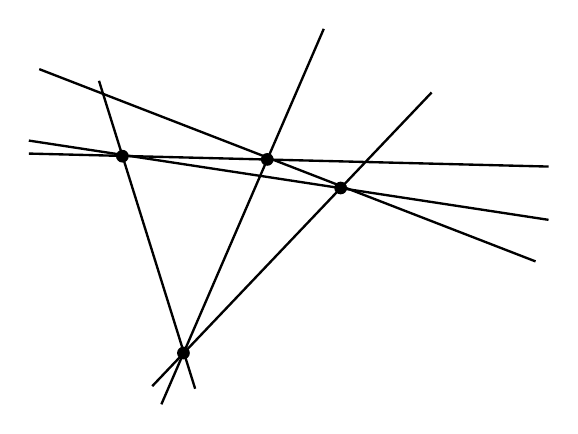
\begin{tikzpicture}[x=1.65cm,y=1.65cm,line width=.85pt]
  \coordinate (A) at (.72,1.87);
  \coordinate (B) at (1.835,1.845);
  \coordinate (C) at (2.4,1.625);
  \coordinate (D) at (1.19,.355);
  \draw (0,1.89)--(4,1.79);       %
  \draw (0,1.99)--(4,1.38);       %
  \draw (.54,2.45)--(1.28,.08);   %
  \draw (.08,2.54)--(3.9,1.06);   %
  \draw (2.27,2.85)--(1.02,-.04); %
  \draw (3.10,2.36)--(.95,.10);   %
  \foreach \p in {A,B,C,D} \fill (\p) circle (2.3pt);
\end{tikzpicture}

  \caption{四个一般位置的点确定的三对直线。}\label{fig:D-7-6}
\end{figure}
\[
  \overline{\mathcal M}_{0,5}
  \cong(S^2\times S^2)\#3\overline{\mathbb CP}^{2}
  \cong\mathbb CP^2\#4\overline{\mathbb CP}^{2}.
\]

类似构造还可用来研究复结构固定的高亏格曲面上\BookRecordIndex{T0066}标记点的\BookRecordIndex{T0246}模空间。具体地，固定亏格 $g\ge1$ 的黎曼曲面 $\Sigma$，记其复结构为 $j_\Sigma$。那么，在固定复结构 $j_\Sigma$ 的 $\Sigma$ 上取三个点所得的紧化\BookRecordIndex{T0246}模空间 $\overline{\mathcal M}_{g,3}(j_\Sigma)$，微分同胚于一个以 $\Sigma$ 为底空间的纤维丛，其在 $z\in\Sigma$ 上的纤维是将 $\Sigma\times\Sigma$ 在点 $(z,z)$ 处吹起后的空间。因此有\BookRecordIndex{T0279}纤维化
\[
  (\Sigma\times\Sigma)\#\overline{\mathbb CP}^{2}
  \hookrightarrow\overline{\mathcal M}_{g,3}(j_\Sigma)
  \longrightarrow\Sigma.
\]
等价地，$\overline{\mathcal M}_{g,3}(j_\Sigma)$ 自然微分同胚于把三重积 $\Sigma\times\Sigma\times\Sigma$ 沿对角线 $\Delta=\{(z,z,z)\mid z\in\Sigma\}$ 吹起后的空间。利用本附录的构造，可以将 $\overline{\mathcal M}_{g,n}(j_\Sigma)$ 作为子流形嵌入 $\bigl(\overline{\mathcal M}_{g,3}(j_\Sigma)\bigr)^N$，其中 $N=\binom n3$。这个嵌入是 Fulton 和 MacPherson 在文献~\srcite{132} 中对高维代数簇所作构造的一个特例。对任意复流形 $X$，他们把 $X_3$ 定义为将 $X\times X\times X$ 沿对角线 $\Delta=\{(x,x,x)\mid x\in X\}$ 吹起后的空间，然后考虑 $X$ 中 $n$ 个有序互异点的配置空间到 $(X_3)^N$ 的自然嵌入，并证明其像的闭包是光滑子流形。

\paragraph{\BookRecordIndex{T0039}Mumford 商。}
考察 $\overline{\mathcal M}_{0,n}$ 与 $X=(S^2)^n$ 在 $G=\mathrm{SO}(3)$ 对角作用下的 Marsden--Weinstein 商 $X/\!/G$ 的关系，是很有意思的。该作用是 Hamilton 作用。对每个因子，\BookRecordIndex{T0204}矩映射为把单位球面 $S^2$ 包含进 $\mathbb R^3\cong\mathfrak{so}(3)$ 的映射~\srcite{293}。因此，$X$ 上 $\mathrm{SO}(3)$ 作用的\BookRecordIndex{T0204}矩映射 $\mu:X\to\mathbb R^3$ 为
\[
  \mu(x_1,\ldots,x_n)=x_1+\cdots+x_n.
\]
从而 $\mu^{-1}(0)$ 是 $(S^2)^n$ 中平均值为零的 $n$ 元组 $(x_1,\ldots,x_n)$ 的集合。\BookRecordIndex{T0204}矩映射的\BookRecordIndex{T0233}临界点是所有向量 $x_i\in\mathbb R^3$ 两两线性相关、因而位于一条过原点直线上的 $n$ 元组。所以，$0$ 是 $\mu$ 的\BookRecordIndex{T0409}正则值，当且仅当 $n$ 为奇数。此外，要使 $G=\mathrm{SO}(3)$ 在 $\mu^{-1}(0)$ 上自由作用，每个 $n$ 元组中至少须有三个互异的 $x_i$。当 $n$ 为偶数时，这两个条件都不满足：$\mu^{-1}(0)$ 在恰有一半 $x_i$ 等于 $a$、另一半等于 $-a$ 的点处奇异，且 $G$ 在这些点处的作用并不自由。另一方面，当 $n$ 为奇数时，Marsden--Weinstein 商
\[
  X/\!/G:=\mu^{-1}(0)/G
\]
是紧致光滑\BookRecordIndex{T0358}辛流形，也称为\emph{约化空间}。

Kirwan 在文献~\srcite{293} 中证明，在这里这样的良好情形下，辛商 $X/\!/G$ 可与几何不变量理论中由复化群 $G^c$ 的作用定义的所谓 $X$ 的 \BookRecordIndex{T0039}Mumford 商等同。习题~\ref{ex:D-7-1} 表明，通常的商 $X/G^c$ 可能性质很差。Mumford 发现，$X$ 中有所谓\emph{半稳定点}构成的子集 $X^{ss}$，在良好情形下其商 $X^{ss}/G^c$ 是紧致光滑流形。一般说来，复几何中的 \BookRecordIndex{T0039}Mumford 商构造相当微妙，这里不予讨论。在辛几何中，若一点的复化群轨道的闭包与 $\mu^{-1}(0)$ 相交，就称它为\emph{半稳定}；若该轨道本身与 $\mu^{-1}(0)$ 相交，就称它为\emph{\BookRecordIndex{T0114}多重稳定}；若它\BookRecordIndex{T0114}多重稳定且其\BookRecordIndex{T0342}稳定子群有限，就称它为\emph{稳定}。半稳定点和稳定点分别构成 $X$ 的开子集，复商 $X^{ps}/G^c$ 自然同构于辛商 $X/\!/G$。所谓良好情形，是指 $0$ 是\BookRecordIndex{T0204}矩映射的\BookRecordIndex{T0409}正则值且 $G$ 在 $\mu^{-1}(0)$ 上自由作用。此时辛商是光滑流形（若\BookRecordIndex{T0204}矩映射恰当，则还紧致），每个半稳定点都是稳定点，Kirwan 定理给出辛商与复商的自然等同：
\[
  X/\!/G\cong X^s/G^c.
\]

在这里，复化群 $G^c=\mathrm{PSL}(2,\mathbb C)$ 通过 \BookRecordIndex{T0040}Möbius 变换在 $X=(S^2)^n$ 上作对角作用。$n$ 元组 $\mathbf z=(z_1,\ldots,z_n)\in X$ 半稳定，当且仅当至多 $n/2$ 个 $z_i$ 相等，即
\[
  X^{ss}=\{\mathbf z\in(S^2)^n\mid
  \text{若 }z_{i_1}=\cdots=z_{i_m},\ i_1<\cdots<i_m,
  \text{ 则 }2m\le n\}.
\]
它稳定，当且仅当少于 $n/2$ 个 $z_i$ 相等，即
\[
  X^s=\{\mathbf z\in(S^2)^n\mid
  \text{若 }z_{i_1}=\cdots=z_{i_m},\ i_1<\cdots<i_m,
  \text{ 则 }2m<n\}.
\]
它\BookRecordIndex{T0114}多重稳定，当且仅当它稳定，或者恰有两个点各出现 $n/2$ 次。当 $n$ 为偶数时，商 $X^{ss}/G^c$ 甚至不是 Hausdorff 空间，而 $X^s/G^c$ 虽是光滑流形，却不紧致，也不与 $X/\!/G$ 微分同胚。另一方面，若 $n\ge3$ 为奇数，则 $X^{ss}=X^{ps}=X^s$，商 $X^s/G^c$ 是维数 $2n-6$ 的紧致光滑流形，且与 $X/\!/G$ 微分同胚。

现在注意，\BookRecordIndex{T0246}模空间 $\overline{\mathcal M}_{0,n}$ 的开\BookRecordIndex{T0072}层 $\mathcal M_{0,n}=((S^2)^n\setminus\Delta_n)/G^c$ 可嵌入 $X^s/G^c$。当 $n$ 为奇数时，这个包含映射延拓为自然投影
\[
  \overline{\mathcal M}_{0,n}\longrightarrow X^s/G^c.
\]
下面给出 Mukai 向我们说明的显式描述。设 $\mathbf z=(\{z_{\alpha\beta}\}_{\alpha E\beta},\{\alpha_i,z_i\}_{1\le i\le n})$ 是以树 $T$ 为模型的\BookRecordIndex{T0339}稳定曲线。若 $(z_{\alpha1},\ldots,z_{\alpha n})\in X^s$，就称 $\alpha$ 为 $T$ 的\emph{\BookRecordIndex{T0038}Mumford 分量}。当 $n$ 为奇数时，每条\BookRecordIndex{T0339}稳定曲线 $\mathbf z$ 都有唯一的 \BookRecordIndex{T0038}Mumford 分量 $\alpha_{\mathbf z}$（试证之！）。所得映射 $[\mathbf z]\mapsto[z_{\alpha_{\mathbf z}1},\ldots,z_{\alpha_{\mathbf z}n}]$ 是光滑的。当 $n=3$ 或 $5$ 时，它是微分同胚；当 $n>5$ 时则不是。因此，若 $n$ 为奇数，$\mathcal M_{0,n}$ 的 Grothendieck--Knudsen 紧化 $\overline{\mathcal M}_{0,n}$ 是 \BookRecordIndex{T0039}Mumford 商 $(S^2)^n/\!/\mathrm{SO}(3)$ 的加细。

\begin{exercise}\label{ex:D-7-1}
如上设 $X=(\mathbb CP^1)^n$、$X^{ss}$、$G^c=\mathrm{PSL}(2,\mathbb C)$。直接证明，对每个 $n$，$X^{ss}/G^c$ 都紧致，尽管 $X^{ss}$ 不紧致。证明 $X/G^c$ 上的商拓扑不是 Hausdorff 拓扑。\emph{提示：}考虑 $z_1=\cdots=z_n$ 的点 $\mathbf z=(z_1,\ldots,z_n)$ 的轨道。证明 $\mathbf z$ 的等价类在 $X/G^c$ 中唯一的邻域是整个空间。
\end{exercise}

\begin{exercise}\label{ex:D-7-2}
证明映射 $\mathcal M_{0,6}\to X^{ss}/G^c$ 不能连续延拓到 $\overline{\mathcal M}_{0,6}$。证明当偶数 $n>4$ 时，$X^{ss}/G^c$ 非 Hausdorff。证明当 $n$ 为奇数时，映射 $\overline{\mathcal M}_{0,n}\to X^{ss}/G^c$ 定义良好。证明它在 $n=5$ 时是微分同胚，但在 $n=7$ 时不是。
\end{exercise}

\paragraph{文献评述。}
空间 $\overline{\mathcal M}_{0,n}$ 最早由 Grothendieck 和 Knudsen 发现。相应的高亏格曲线\BookRecordIndex{T0246}模空间 $\overline{\mathcal M}_{g,n}$ 由 Deligne 和 Mumford 构造。Knudsen 在文献~\srcite{211} 中证明，$\overline{\mathcal M}_{0,n}$ 是光滑射影代数簇。Kapranov 在文献~\srcite{206} 中，将 $\overline{\mathcal M}_{0,n}$ 描述为复 Grassmann 流形 $G(2,n)$ 关于极大环面 $H\subset\mathrm{GL}(n,\mathbb C)$ 的 Chow 商。他还把该\BookRecordIndex{T0246}模空间表示为一个吹起。Keel 在文献~\srcite{208} 中计算 $\overline{\mathcal M}_{0,n}$ 的上同调环，并证明它与 Chow 环同构。

与本附录类似的构造，也见于 Naraki 对 $\mathbb CP^3$ 中三次曲面的研究（参见文献~\srcite{297}）。每个这样的三次曲面 $S\subset\mathbb CP^3$ 包含 $27$ 条直线；对 $S$ 中每条直线 $L$，恰有五个平面 $H\subset\mathbb CP^3$ 同时包含 $L$ 与 $S$ 中另两条直线。从这五个平面中任取四个，即得一个\BookRecordIndex{T0185}交比：取与这四个平面都横截的任意直线 $L'$，它与四个平面的四个交点的\BookRecordIndex{T0185}交比与 $L'$ 的选取无关。这样产生 $135$ 个\BookRecordIndex{T0185}交比，其中 $45$ 个独立。Naraki 证明，这个构造把带 $27$ 条直线之排序的 $\mathbb CP^3$ 中三次曲面\BookRecordIndex{T0246}模空间嵌入 $45$ 份 $\mathbb CP^1$ 的乘积。
